\section{Divisor-interval laws}\label{sec:interval}
Edges and cells of the move complex are decided by a local arithmetic test on divisor intervals; this turns the transition between consecutive complexes into a statement about which new occurrences fall into which old intervals.

\subsection{The edge rule}
For occurrences $u,v\in D$ write $[u,v]^\circ=\{w\in\N:\gcd(u,v)\mid w\mid\lcm(u,v)\}$ for the \emph{divisor interval}; in exponent coordinates it is the coordinate hull $H(e(u),e(v))$, with $1\leftrightarrow0$.
\begin{theorem}[divisor-interval rule]\label{thm:A5T31}
Two distinct occurrences $u,v\in D(x)$ are joined by an edge of $\Kmove(x)$ if and only if $[u,v]^\circ\cap(D\cup\{1\})=\{u,v\}$. In particular $\Kmove(x)$ is a function of $D(x)$ alone: the denominator $b$ enters only through which $D$ occurs.
\end{theorem}
\prov{CW-0441}{A5-T3.1}{PROVED}{FULL}
\begin{proof}
The $1$-cells of $\Kmove$ are the pairs $\{w,w+g\}\subseteq F$ with $g\in\Gr(x)$. By \cref{lem:hull} (with $u=e(u)$, $v=e(v)$), $v-u\in\Gr(x)$ iff the coordinate hull contains no point of $F\cup\{0\}$ other than the endpoints. Under the bijection $F\leftrightarrow D$, $0\leftrightarrow1$, the hull is $[u,v]^\circ$. \qedhere
\end{proof}
\begin{definition}[$K(D)$ for an arbitrary set]\label{def:KD}
For any finite $D\subset\N_{\ge2}$ let $K(D)$ be the cell complex with vertex set $D$, edges given by the rule of \cref{thm:A5T31}, and cells the parallelotopes $P(u;g_1,\dots,g_j)$ (lexicographically positive, linearly independent generators in the universal coordinates) all of whose $2^j$ vertices lie in $D$ and all of whose $1$-faces are edges.
\end{definition}
\begin{proposition}[intrinsic-Graver lemma]\label{prop:intrinsic}
For every state $x$, $\Kmove(x)=K(D(x))$.
\end{proposition}
\begin{proof}
A cell $P(u;g_1,\dots,g_j)$ of $\Kmove(x)$ has all vertices in $F$ and $g_i\in\Gr(x)$; its $1$-faces are the pairs $\{w,w+g_i\}\subseteq F$, which are edges by \cref{lem:hull}. Conversely if all vertices lie in $F$ and all $1$-faces are edges, then each generator $g_i=(w+g_i)-w$ with both endpoints in $F$ and $\{w,w+g_i\}$ an edge lies in $\Gr(x)$ (\cref{lem:hull}). \qedhere
\end{proof}
\begin{remark}[independent confirmation; finite-exact]
The equality was checked in the source release, with identical $f$-vectors and Betti numbers over $\F_2$ and over a large prime field, against an engine building $\Kmove$ from the lattice rather than from $D$, on $1{,}783$ states (towers, orbits for $\ell=5,7,11,13$, the activation family); that check is inherited and \stat{cited}. In the present paper the edge sets of $K(D)$ from the divisor-interval rule and from the lattice region-Graver routine were compared on $182$ states (the first $30$ steps of the orbits of $3025/3$, $126^2/5$, $1890^2/29$, $36^2/5$, $176^2/7$ and $S_0^2/11$ for $S_0=2^23^35^4$, numerators below $10^{13}$) with no mismatch (\stat{finite-exact}; script \texttt{xcheck\_KD.py}).
\end{remark}
\begin{corollary}[local consequences of the rule]\label{cor:local}
\begin{enumerate}[label=(\alph*),itemsep=1pt]
\item \emph{Coprime non-adjacency.} If $\gcd(u,v)=1$ there is no edge $\{u,v\}$, since $1\in[u,v]^\circ$.
\item \emph{Comparable pairs.} If $u\mid v$, then $\{u,v\}$ is an edge iff $u$ and $v$ are consecutive in the divisibility order of $D\cup\{1\}$.
\item \emph{Positive-primitive moves.} A positive vector $e(d)$, $d\in D$, belongs to $\Gr(x)$ iff $d$ is divisibility-minimal in $D$.
\end{enumerate}
\end{corollary}
\begin{proof}
(a) is immediate. (b) $[u,v]^\circ=\{w:u\mid w\mid v\}$. (c) The proof of \cref{lem:hull} applies with $u=0$ ($h\sqsubseteq e(d)$, $h\ne0,e(d)$, $h\in\Lambda_b$ is a point of $F$, i.e.\ a proper divisor of $d$ in $D$). \qedhere
\end{proof}

\subsection{The transition law}
Let $D\subseteq D'$ be finite sets, $N=D'\setminus D$, $K=K(D)$, $K'=K(D')$. An edge of $K$ is \emph{dead} (for $D'$) if it is not an edge of $K'$; a cell of $K$ is \emph{dead} if one of its edges is. Put $\mathrm{Dead}=\{\text{dead cells of }K\}$, $K^\circ=K\cap K'$, $\mathrm{New}=K'\setminus K$ (cells).
\begin{theorem}[transition law]\label{thm:A5T32}
\begin{enumerate}[label=(\arabic*),itemsep=1pt]
\item \emph{Non-edges persist}: a pair of $D$ that is not an edge of $K$ is not an edge of $K'$.
\item \emph{An old edge $\{u,v\}$ is dead iff some $w\in N$ lies in $[u,v]^\circ$.}
\item \emph{Every new edge and every new cell contains a new vertex.}
\item A cell dies iff one of its edges dies.
\item $K^\circ=K\setminus\mathrm{Dead}$ is a subcomplex of both $K$ and $K'$, and $K'=K^\circ\cup\mathrm{New}$.
\item \emph{Moves.} A realised move $g=e(v)-e(u)$ disappears iff every pair realising it is dead; it can appear only through a pair containing a new vertex. Consequently if $N\ne\emptyset$ is not met, no move changes: vertex growth is necessary for any change, edge loss needs a piercing new occurrence, and a new $2$-cell needs a new vertex.
\end{enumerate}
\end{theorem}
\prov{CW-0442}{A5-T3.2}{PROVED}{FULL}
\begin{proof}
(1) A non-edge $\{u,v\}$ has a point $w\in[u,v]^\circ\cap(D\cup\{1\})$, $w\ne u,v$; as $D\cup\{1\}\subseteq D'\cup\{1\}$ it is still a non-edge. (2) An old edge has no point of $D\cup\{1\}$ in its interval other than $u,v$; it is an edge of $K'$ iff there is no point of $D'\cup\{1\}$ there, i.e.\ iff no point of $N$. (3) Let $\{u,v\}$ be an edge of $K'$ with $u,v\in D$: by (1) it is an edge of $K$, so it is not new. If a cell of $K'$ has all vertices in $D$, its $1$-faces are edges of $K'$ between old vertices, hence edges of $K$, so the cell is a cell of $K$. (4) is the definition of cells of $K(D)$ via their $1$-faces. (5) The faces of a surviving cell have fewer edges, all alive, so $K\setminus\mathrm{Dead}$ is a subcomplex of $K$; a cell lies in $K'$ iff its vertices are in $D'$ and its $1$-faces are edges of $K'$, so the cells of $K$ in $K'$ are exactly the surviving ones, and the cells of $K'$ are either of $K$ (surviving) or new. (6) Disappearance and appearance of $g$ follow from (2) and (3). \qedhere
\end{proof}
\begin{corollary}[event localisation]\label{cor:localise}
At the end $\tau$ of a plateau starting at $x_0$, $N=\{d\notin D_0:Q(d)\mid Y_\tau\}$ and the dead edges are $\{\{u,v\}\in E(K(D_0)):\exists\,d\in N,\ \gcd(u,v)\mid d\mid\lcm(u,v)\}$. Both are computed from the \emph{old} complex and the congruence data of the stage; the new complex need not be built.
\end{corollary}
\prov{CW-0443}{A5-T3.3}{PROVED}{FULL}
\begin{proof}
\Cref{cor:event} gives $N$; \cref{thm:A5T32}(2) gives the dead edges. \qedhere
\end{proof}
\begin{example}[a piercing event]\label{ex:interval}
Let $D=\{8,22,176\}$, the occurrence set of $176^2/7$ at step $5$ of its orbit, and $D'=\{2,4,8,11,16,22,44,88,176\}$ at step $6$ ($N=\{2,4,11,16,44,88\}$). The three old edges are $\{8,22\}$, $\{8,176\}$, $\{22,176\}$; the intervals are $\{2,4,8,22,44,88\}$, $\{8,16,88,176\}$ and $\{22,44,88,176\}$, each of which contains a new occurrence ($2$, $16$, $44$ respectively). All three die (\cref{fig:interval}), and $K'$ has $9$ vertices, $11$ edges and $3$ squares (\cref{fig:beforeafter}).
\end{example}
\begin{figure}[tbp]\centering
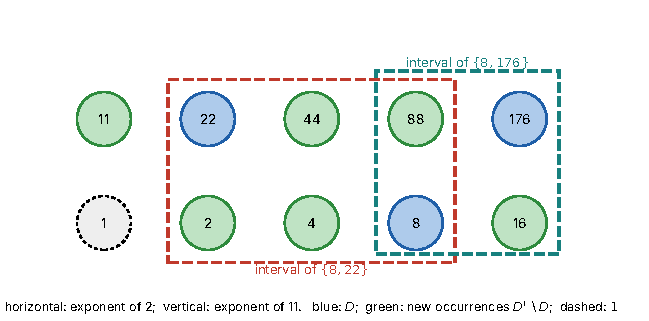
\includegraphics[width=\textwidth]{fig18_divisor_interval}
\caption{\textbf{Divisor intervals pierced by new occurrences (exact; \cref{ex:interval}, proved by \cref{thm:A5T32}).} The nine occurrences in exponent coordinates (horizontal: exponent of $2$; vertical: exponent of $11$). Blue: $D=\{8,22,176\}$ at step $5$ of the orbit of $176^2/7$; green: the new occurrences at step $6$; dashed circle: $1$. The dashed boxes are the intervals of $\{8,22\}$ and $\{8,176\}$; each contains a new occurrence. The interval of $\{22,176\}$ is pierced likewise.}\label{fig:interval}
\end{figure}
\begin{figure}[tbp]\centering
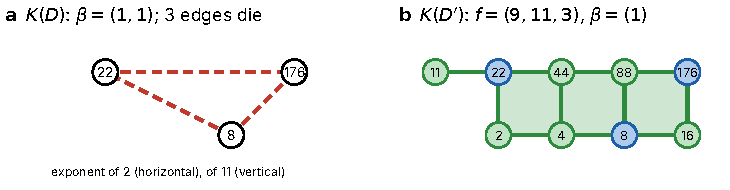
\includegraphics[width=\textwidth]{fig19_before_after}
\caption{\textbf{Before and after the same event (exact; \cref{ex:interval}).} Both complexes are drawn in exponent coordinates $(v_2,v_{11})$, a genuine planar embedding of the grid complex. (a) $K(D)$: three vertices, three dashed edges that will die, $\beta=(1,1)$. (b) $K(D')$: $9$ vertices, $11$ edges, three squares (shaded), $\beta=(1,0)$; the new edges are drawn in green. The abstract reading (which edges died) is the content of \cref{thm:A5T32}; the geometric reading is the picture.}\label{fig:beforeafter}
\end{figure}
